\section{Interchanging and Stacking VOL Plugins}
\label{sec:stack}

Accessing an HDF5 container with a VOL plugin different than the one
it was created with would be a valid approach as long as the
underlying file format is the same. This would be the user’s
responsibility to ensure that the different plugins are
interchangeable.

\subsection{Stacking Plugins on Top of Each Other}
It would be also possible to stack VOL plugins on top of each
other. This notion is similar to the idea of the split VFD, where
underneath the split VFD itself, two file drivers would be used, one
for the file storing the metadata and another for raw data. Some
stackings make sense and others would be erroneous. For example,
stacking the native HDF5 plugin on top of a non-HDF5 backend plugin
does not make sense and is erroneous. Figure~\ref{fig:stack} shows a
stacking of a remote plugin, where data is distributed remotely, on
top of the native h5 plugin, where servers that store the data at
remote locations use the h5 file format.

\begin{figure}[ht!]
\centering
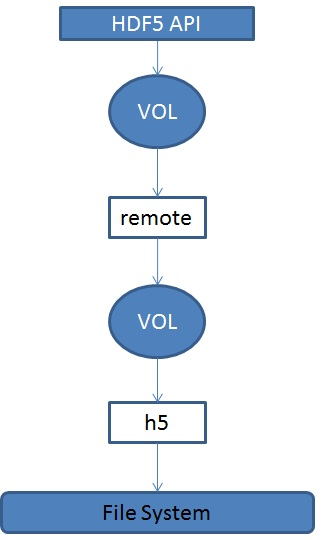
\includegraphics[width=90mm]{stacked.jpg}
\caption{Stacked VOL plugins.}
\label{fig:stack}
\end{figure}

\subsection{Mirroring Plugins}
Another useful design option is to allow a mirroring plugin, where the
HDF5 API calls are forwarded through a mirror plugin to two or more
VOL plugins. This is an extention to the stacking
feature. Figure~\ref{fig:mirror} shows an example of a VOL mirror that
maps HDF5 API calls to an h5 backend plugin and an XML backend plugin.

\begin{figure}[ht!]
\centering
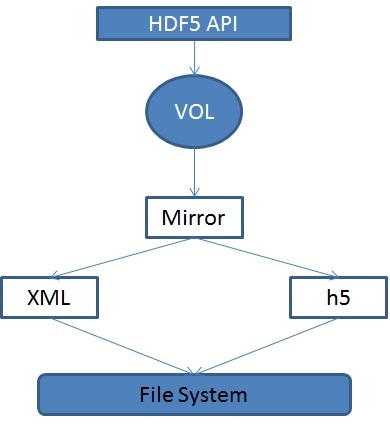
\includegraphics[width=90mm]{mirrored.jpg}
\caption{Mirrored VOL plugins.}
\label{fig:mirror}
\end{figure}

Another possible VOL plugin could be a statistics plugin that just
gathers information on HDF5 API calls and records statistics
associated with the number of calls to a specific API functions and
corresponding parameters. This plugin would be very useful for
profiling purposes. The statistics plugin would be stacked on top of
another VOL plugin that actually performs the required access to the
file.

\subsection{Implementing Stacked and Mirrored Plugins}
A new set of API calls that map directly to the VOL callbacks have
been added to the HDF5 library to make stacking and mirroring easy for
plugin developers. Those APIs are listed at then end of Section~\ref{sec:api}. They are similar to the public VFD (H5FD) routines that call the VFD callbacks directly.

A mirror VOL plugin could, for example, implement the create callback in the file class by creating two HDF5 containers each with a different underlying plugin with 2 calls to:
\begin{lstlisting}
void *H5VLfile_create(const char *name, unsigned flags, hid_t fcpl_id, hid_t fapl_id, hid_t dxpl_id, void **req);
\end{lstlisting}
where each call uses a different file access property list, each with the VOL plugin property set to the underlying plugin. Then the mirror plugin creates a structure containing the pointers for the containers returned from both underlying plugins and returns a pointer to that structure as the output of the file create callback. Subsequent access to the container created would receive as input the structure with the two files and would again call the the public VOL routines twice for each plugin with its corresponding file object and combine the output as needed. 

Appendix~\ref{sec:A} show an example on how to stack a simple plugin that does a printf of the VOL operation on top of the native HDF5 plugin.

\pagebreak

%%% Local Variables: 
%%% mode: latex
%%% TeX-master: t
%%% End: 
